\chapter{Results}
\label{chp4}
In the previous chapter, we have discussed the methodology and the software we have used to implement this code. In this chapter we are presenting the result of our project.
\section{Home Page}
Home page of the project is shown in the following figure.
\begin{figure}[H]  %h=positioning
\begin{center}
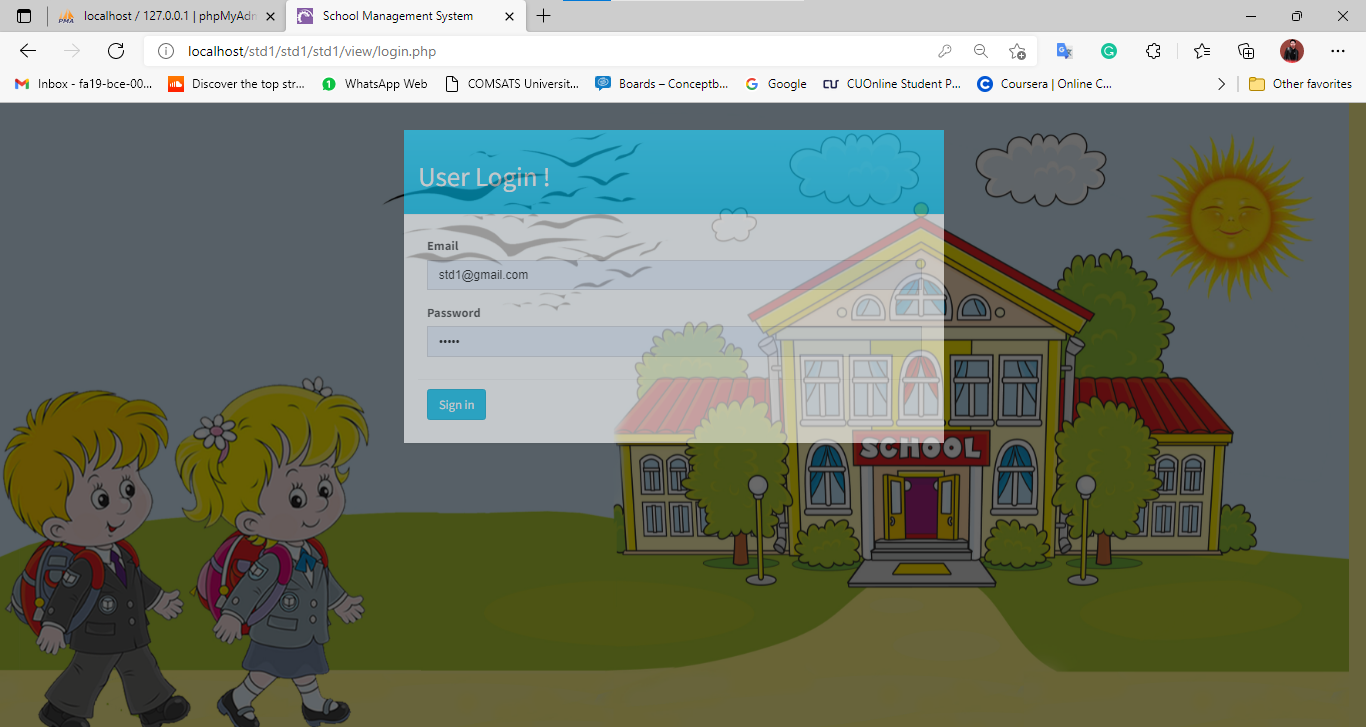
\includegraphics[scale=0.45]{Chapter4/homePage}
\caption{Home Page of SMS}
\label{homePage}
\end{center}
\end{figure}
As we have mentioned in our project feature that it is providing multi login so home page of the school management system is providing us following four (4) login options:
\begin{enumerate}
 \item Admin
 \item Teacher 
 \item Student
 \item Parents
\end{enumerate}
\section{Admin}
We have two admin at the moment but we can add more as much as we want.
\begin{enumerate}
\item email:admin1@gmail.com, password: 12345
\item email:admin2@gmail.com, password: 12345
\end{enumerate}
\begin{figure}[H]  %h=positioning
\begin{center}
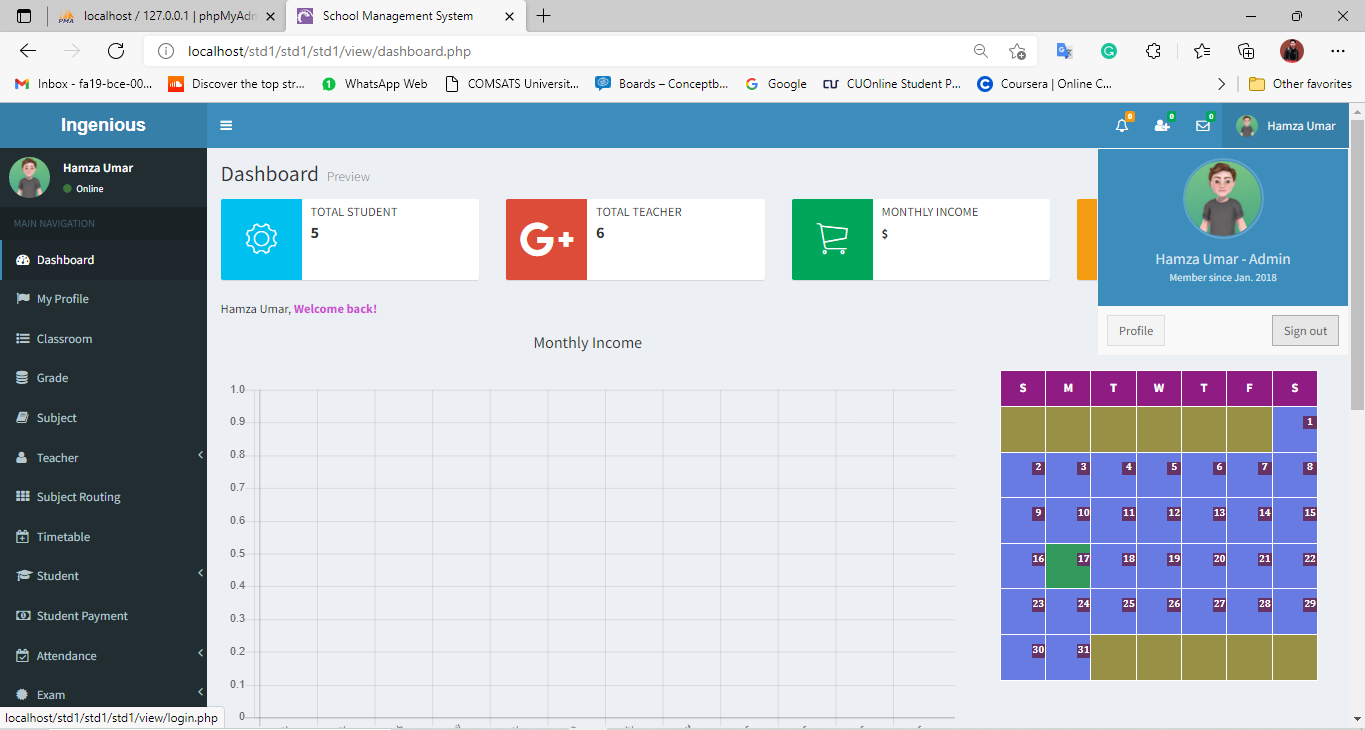
\includegraphics[scale=0.45]{Chapter4/admin1}
\caption{Admin View}
\label{admin1}
\end{center}
\end{figure}
Admin have all the access on the web base school management system and can add and edit everything on the web.
\section{Teacher}
Teacher is having access on the tabs mentioned on the left side of the screen.
We have some teachers at the moment but we can add more as much as we want.
\begin{enumerate}
\item email:t1@gmail.com, password: 12345
\item email:t2@gmail.com, password: 12345
\item email:t3@gmail.com, password: 12345
\item email:t4@gmail.com, password: 12345
\item email:t5@gmail.com, password: 12345
\item email:t6@gmail.com, password: 12345
\end{enumerate}
Following figure is showing a teacher login view.
\begin{figure}[H]  %h=positioning
\begin{center}
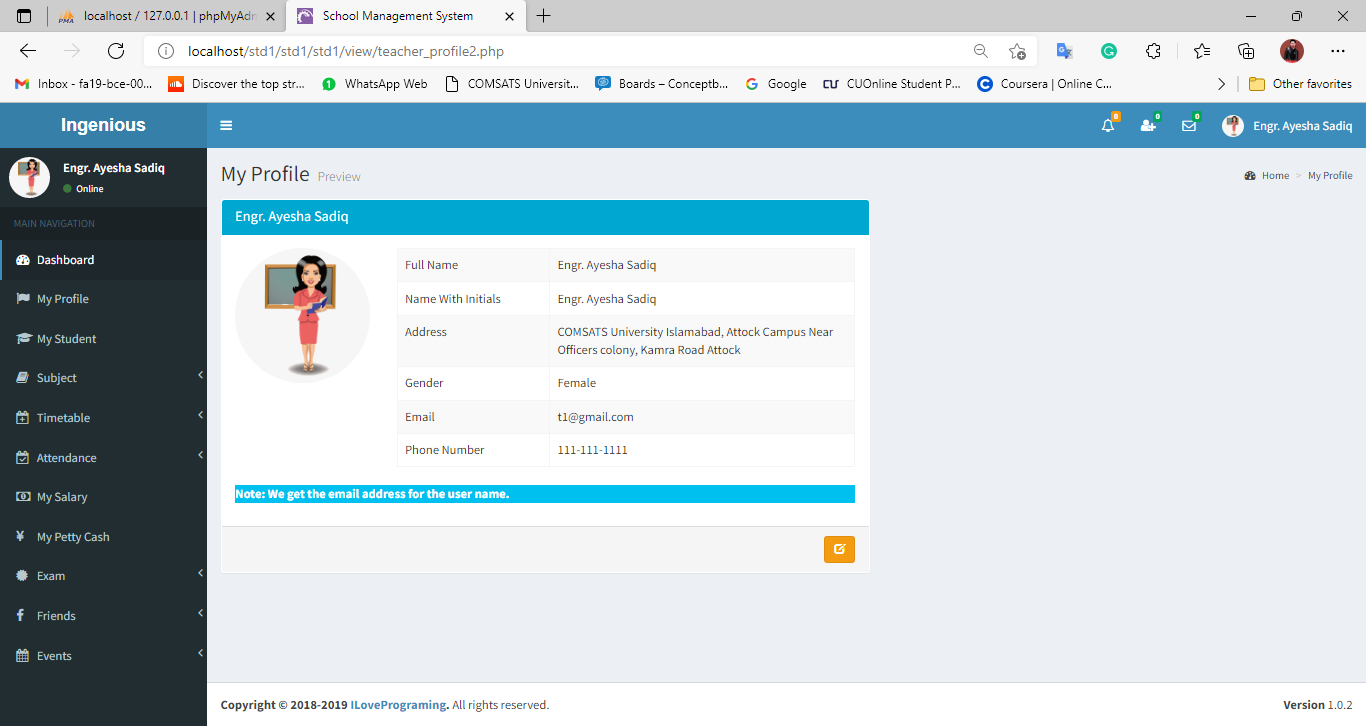
\includegraphics[scale=0.45]{Chapter4/teacher}
\caption{Teacher View}
\label{teacher}
\end{center}
\end{figure}
\section{Student}
A student view is showing in the following figure, a student have some access to the resources given to them by developers.
We have some students at the moment but we can add more as much as we want.
\begin{enumerate}
\item email:std1@gmail.com, password: 12345
\end{enumerate}
\begin{figure}[H]  %h=positioning
\begin{center}
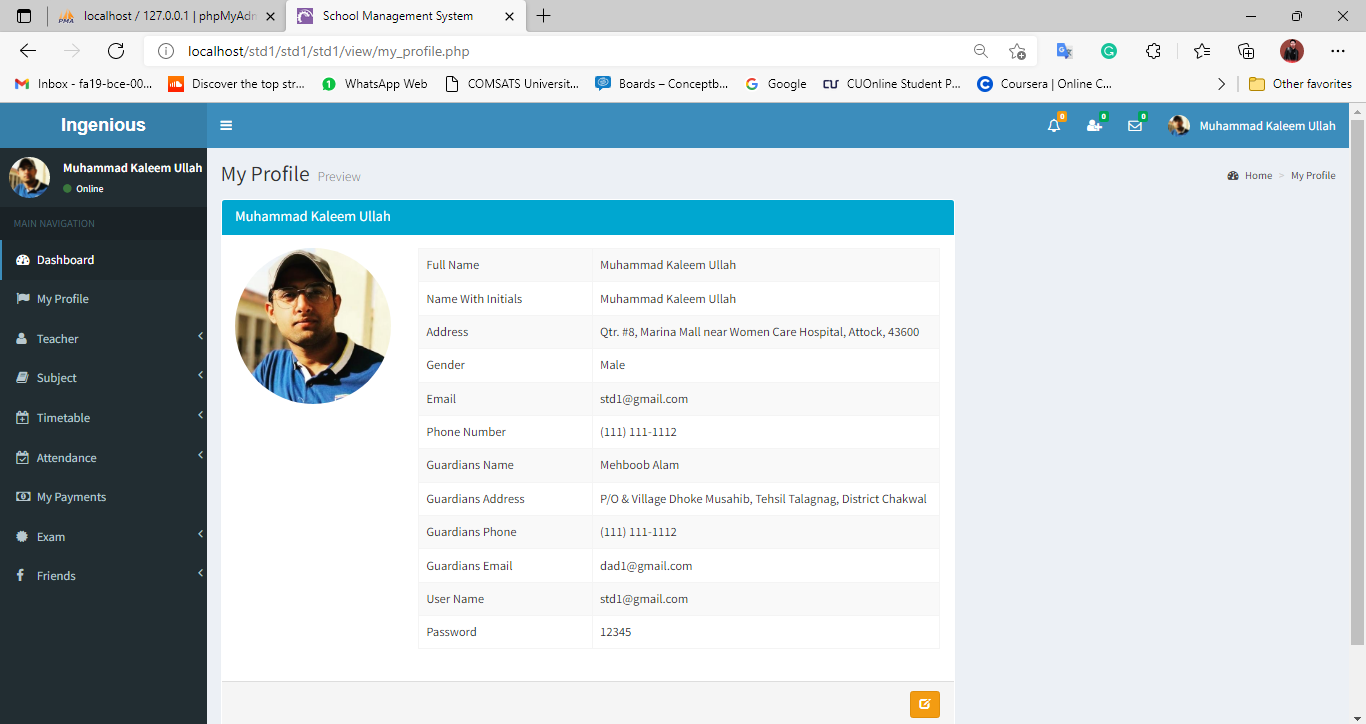
\includegraphics[scale=0.43]{Chapter4/student}
\caption{Student View}
\label{student}
\end{center}
\end{figure}
\section{Parents}
A parent's view is showing in the following figure.
We have some parents at the moment but we can add more as much as we want.
\begin{enumerate}
\item email:dad1@gmail.com, password: 12345
\end{enumerate}
\begin{figure}[H]  %h=positioning
\begin{center}
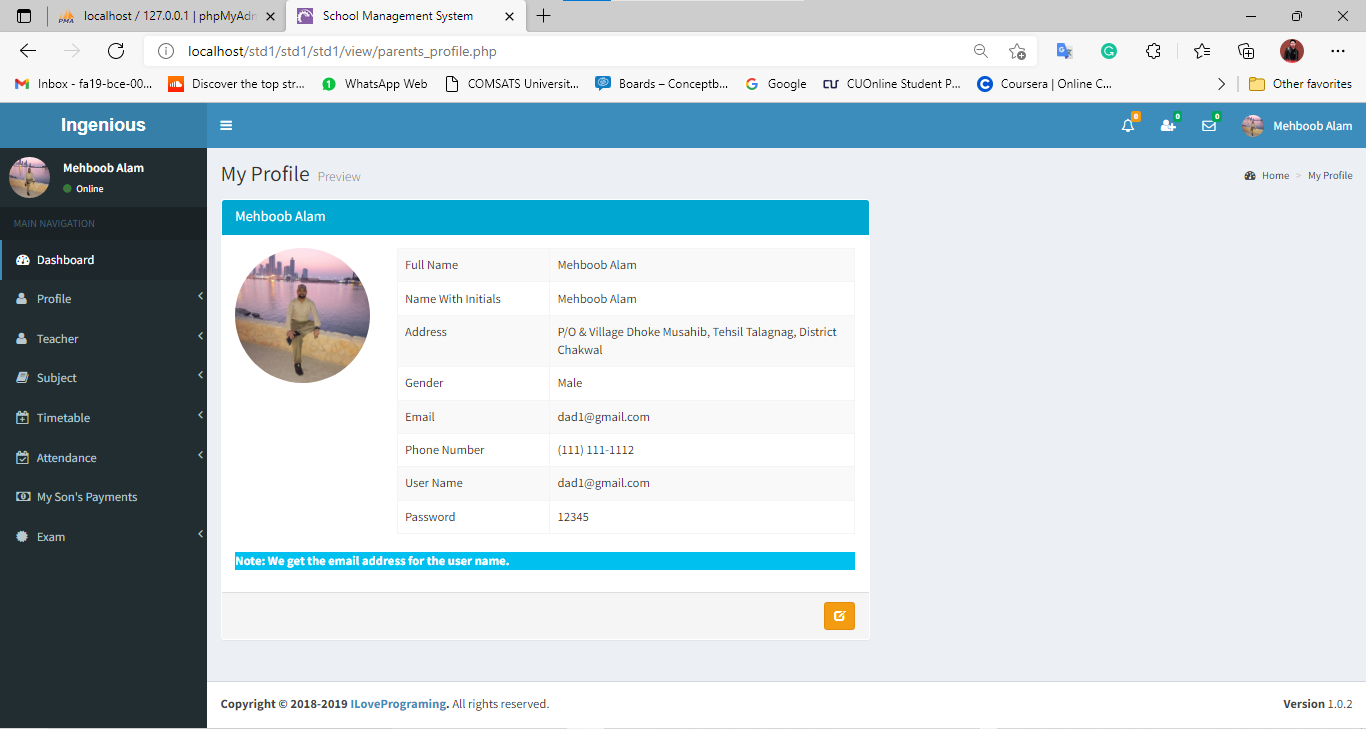
\includegraphics[scale=0.42]{Chapter4/parent}
\caption{Parent View}
\label{parent}
\end{center}
\end{figure}
\section{PHP Admin View}
A phpmyadmin view is showing in the following figure. We can add, edit and can delete at this platform.
\begin{figure}[H]  %h=positioning
\begin{center}
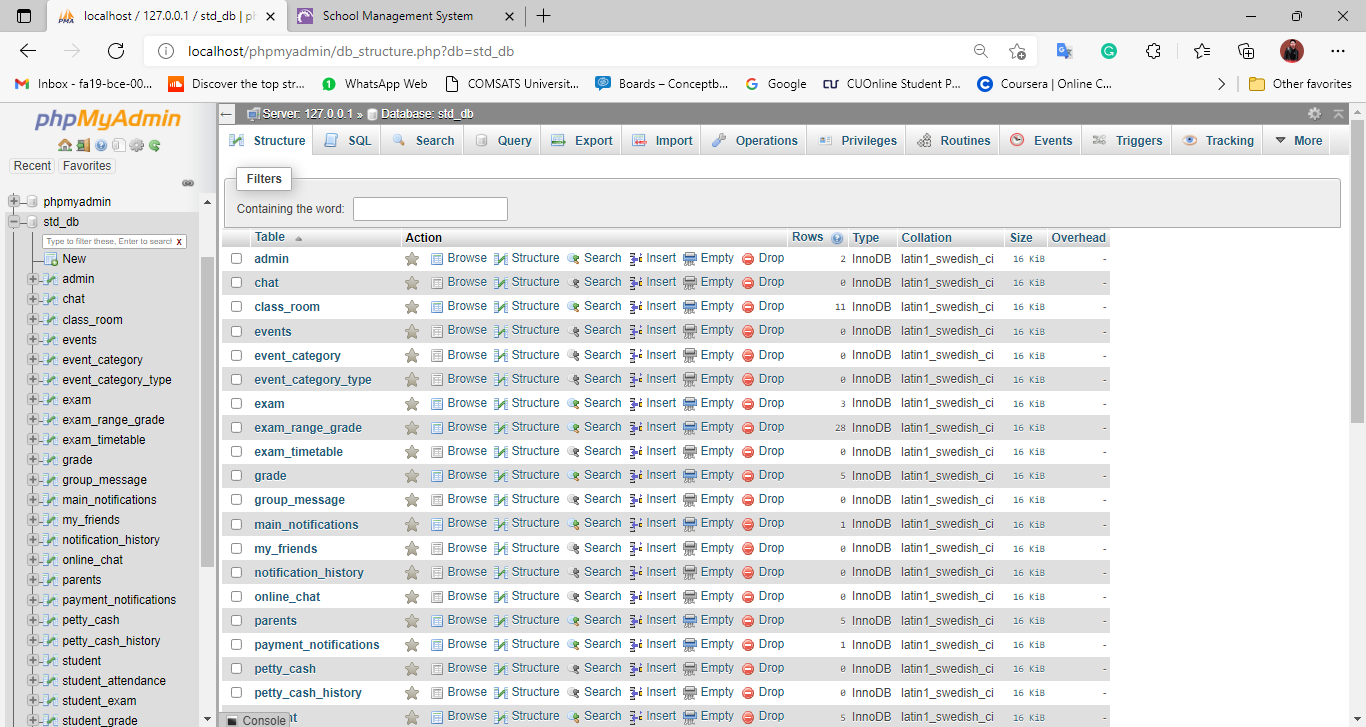
\includegraphics[scale=0.42]{Chapter4/phpadmin}
\caption{phpAdmin View}
\label{parent}
\end{center}
\end{figure}